\documentclass{article}

\usepackage[czech]{babel}
\usepackage[utf8]{inputenc}
\usepackage[T1]{fontenc}

\usepackage[left=2cm,text={17cm, 24cm},top=3cm, bottom=2cm]{geometry}

\usepackage{rotating}
\usepackage{graphicx} % vkládání obrázků
\usepackage{amsmath} % pokročilá sazba matematiky
% \usepackage{xcolor} % barevný text
% \usepackage[european]{circuitikz} % Obvody
\usepackage{siunitx} % SI jednotky
\usepackage{graphicx} % Obrázky
\usepackage{hyperref} % Clicable table of contents
\usepackage{color} % Color for table of contents
\usepackage{float}
\usepackage{lscape}
\usepackage{hyperref} 

\restylefloat{figure}

\hypersetup{
    colorlinks=true, %set true if you want colored links
    linktoc=all, %set to all if you want both sections and subsections linked
    linkcolor=black,  %choose some color if you want links to stand out
}

\graphicspath{ {./images} } % Include image folder

% \begin{figure}[H] 
%     \centering
%     \includegraphics[scale=0.7,keepaspectratio]{2_2}
%     \caption{Měření VA charakteristiky}
%     \label{fig:va_dioda}
% \end{figure} for icluding image

% important things: \[  \], \tau , \approx , \SI{1}{\micro\farad} , \SI{10}{\kohm}
% \begin{table}[H]
% 	\begin{center}
% 		\begin{tabular}{|c|c|c|c|c|c|c|c|c|c|c|c|c|c|} 
% 			\hline
% 			Ud [V] & 0.00 &  0.20 & 0.40 & 0.60 & 0.80 & 1.00 & 1.20 & 1.40 & 1.60 & 1.71 & 1.78 & 1.80 & 1.81\\
% 			\hline
% 			Id [mA] & 0.00 & 0.00 & 0.00 & 0.00 & 0.00 & 0.00 & 0.00 & 0.00 & 0.09 & 0.25 & 0.42 & 0.60 & 0.79 \\
% 			\hline
% 		\end{tabular}
% 		
% 		\caption{Naměřené hodnoty napětí a proudu diodou}
% 	\end{center}
% \end{table}

\begin{document}

% start first page
\clearpage
\begin{titlepage}
	\begin{center}
		\textsc{\LARGE Vysoké Učení Technické v Brně}\\[0.5cm]
		{\LARGE Fakulta informačních technologií }\\[4.0cm]

		\textsc{\LARGE ISS}\\[0.5cm]
		\textsc{\LARGE 2020/2021}\\[3.5cm]

		{\LARGE Projekt}\\[1.0cm]
	\end{center}

	\vfill 

	\begin{flushleft} 
		\large
		Martin Douša (xdousa00)
		\hfill
		Brno, \today
	\end{flushleft}
\end{titlepage}
\thispagestyle{empty}

\newpage
\tableofcontents

\newpage
\listoffigures

\newpage
% end first page

\section{Úvod}

"Casto se stane, ze dostaneme signal zaruseny nejakymi artefakty a je potreba jej vyfiltrovat. Pro tento projekt 
jsme pro Vas pripravili signaly ze zname databaze TIMIT, kam se ale “zatoulaly” ctyri harmonicky vztazene
cosinusovky. Vasim ukolem je signal analyzovat, najit, na kterych frekvencich cosinusovky jsou, navrhnout filtr
nebo filtry pro cisteni signalu a pak signal vycistit."

V tomto projektu se budeme zabývat zkoumáním možností analýzy signálu a jeho filtrací podle zadání.
Dále prozkoumáme možnosti filtrování pomocí neuronových sítí a úskalí této metody.

Tento projekt je zpracován v jazyce python za použití knihoven numpy, scipy a matplotlib. Pro dobrovolnou část projektu kde zkoumáme možnosti filtrace pomocí neuronových sítí je použita knihovna tensorflow.

Projekt je složen z dvou nezávyslých částí. První částí je vypracování zadání a druhou částí je můj výzkum možností filtrace pomocí neuronových sítí.
Řešení části ze zadání lze najít v souboru \textbf{main.ipynb}, soubory \textbf{helpers.py}, \textbf{settings.py}, \textbf{process\textunderscore ai\textunderscore data.py}, \textbf{train\textunderscore ai.py} a \textbf{interface\textunderscore ai.py} patří k testování neuronových sítí.

Soubor \textbf{settings.py} obsahuje nastavení tvorby dat pro neuronovou síť, cesty k datům, parametry trénování, atd.
\textbf{helpers.py} obsahuje pomocné funkce pro zpracování dat a tvorbu dat, pomocné callbacky pro trénování, tvorbu modelu a čtení a předzpracování dat.
\textbf{process\textunderscore ai\textunderscore data.py} zpracovává data a vytváří datasety.
\textbf{train\textunderscore ai.py} vytváří model a trénuje ho.
\textbf{interface\textunderscore ai.py} slouží k interakci s modelem po jeho vytrénování.
\section{Základy}

V této části se podíváme na vstupní zarušený signál, který nám byl přiřazen a jeho vlastnosti.

\begin{figure}[H] 
    \centering
    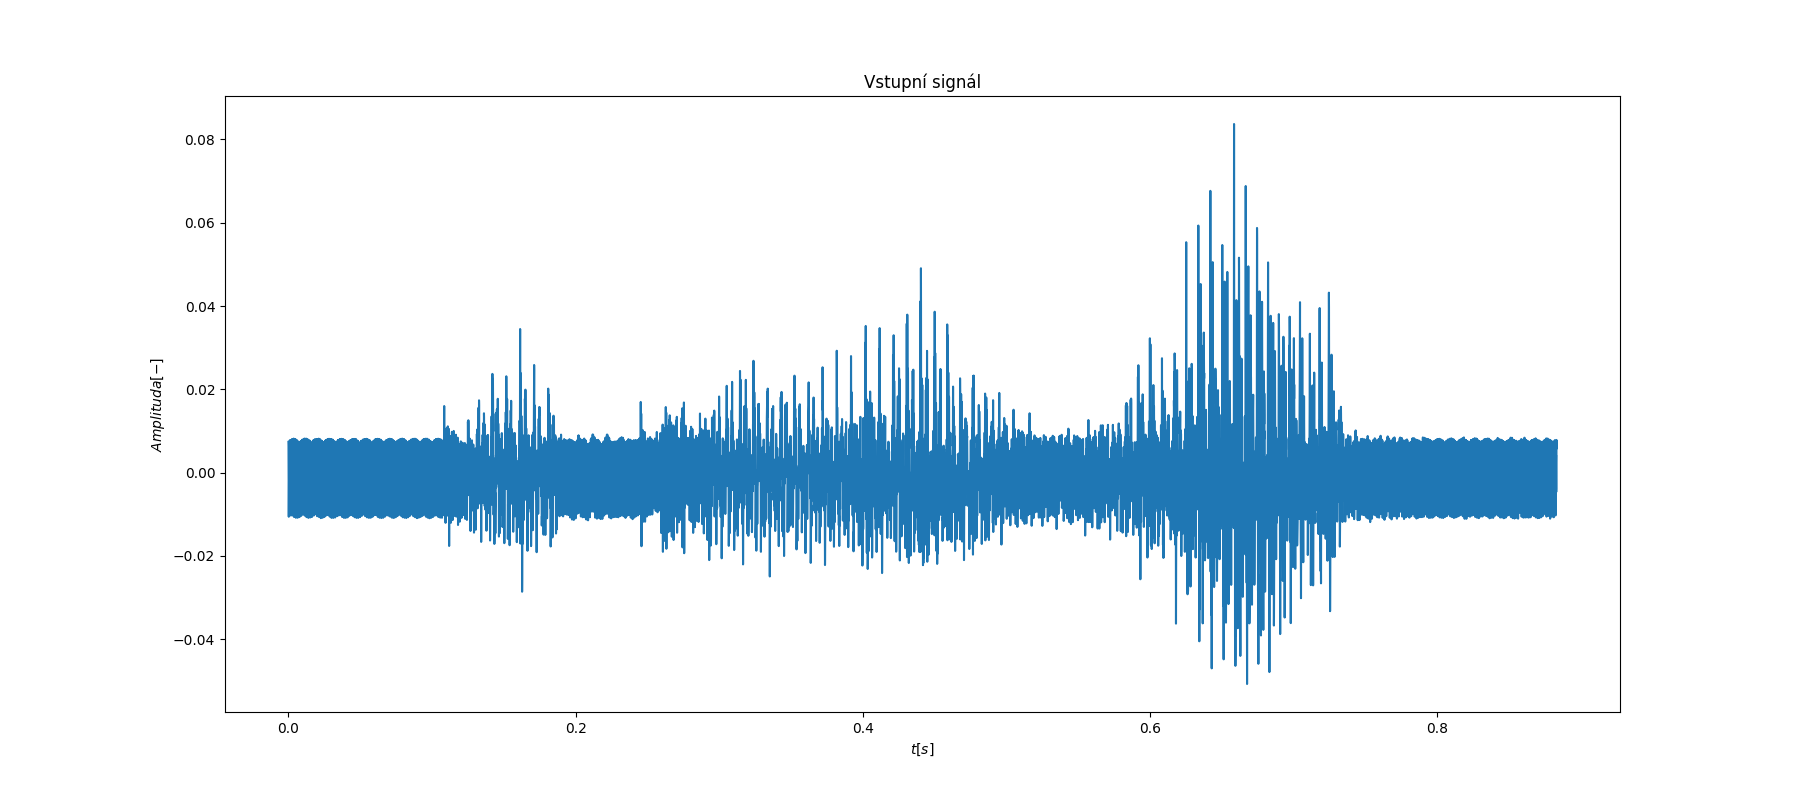
\includegraphics[scale=0.35,keepaspectratio]{Figure_1}
    \caption{Načtený signál}
\end{figure}

Délka vstupního signálu je 14132 vzorků což při vzorkovací frekvenci 16kHz odpovádá 0.88325s.
Maximální hodnota tohoto signálu je přibližně 0.837097 a minimální přibližně -0.050751.
\section{Předzpracování a rámce}

Před tím než začneme pracovat se signálem je hlavní tento signál normalizovat, aby jsme dostali nějaké rozumné hodnoty s kterými pracovat.
Tato část je hlavně důležitá pokud chceme porovávat signály mezi sebou. Další důvod normalizace je pro využité některých algoritmů které neumí pracovat s daty co nejsou normalizované.
Byl zobrazen znělý rámec, v našem případě rámec číslo 11 a jako zajímavost rámec kde je pouze šum a to rámec číslo 0.

\begin{figure}[H] 
	\centering
	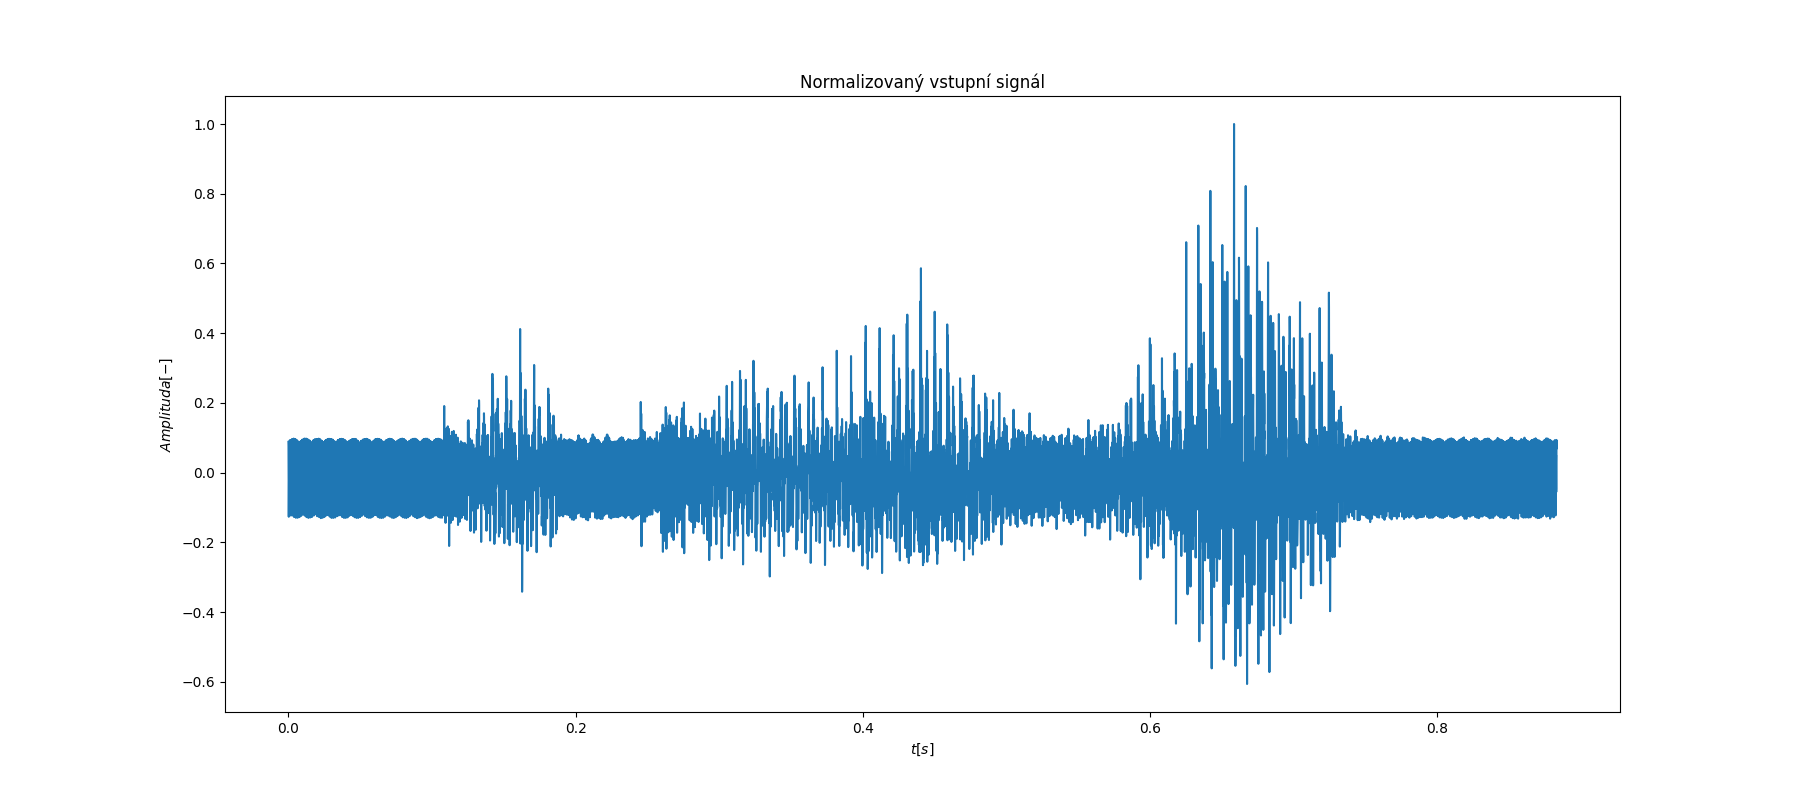
\includegraphics[scale=0.35,keepaspectratio]{Figure_3}
	\caption{Normalizovaný a vycentrovaný vstupní signál}
\end{figure}

\begin{figure}[H] 
	\centering
	\includegraphics[scale=0.35,keepaspectratio]{Figure_43}
	\caption{Vycentrovaný a normalizovaný znělý rámec - rámec \#11}
\end{figure}

\begin{figure}[H] 
	\centering
	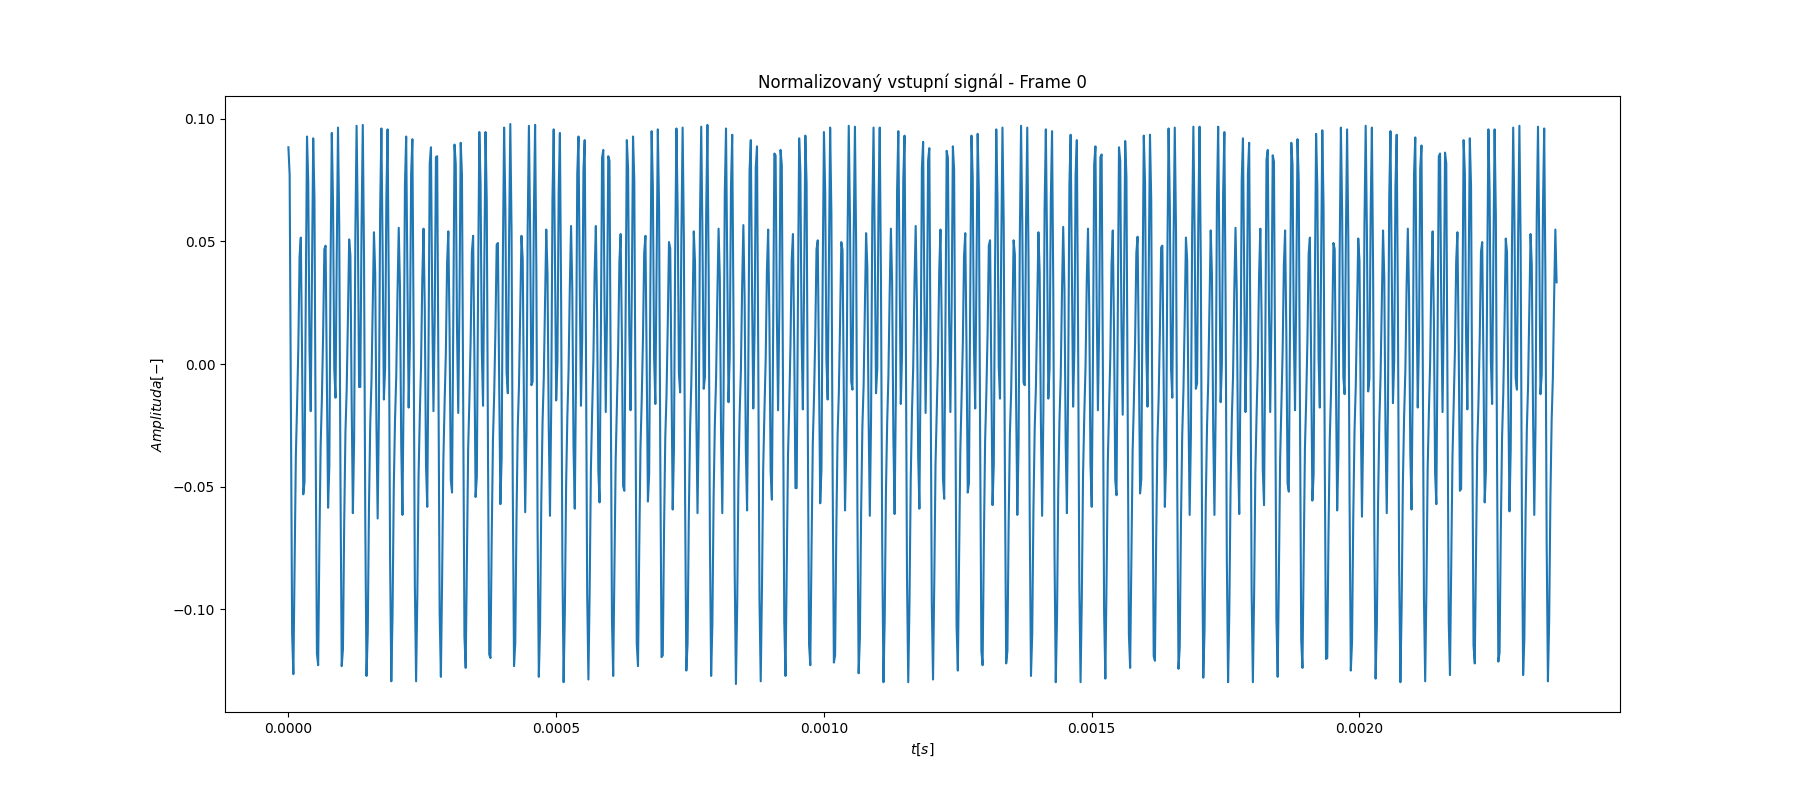
\includegraphics[scale=0.35,keepaspectratio]{Figure_2}
	\caption{Vycentrovaný a normalizovaný rámec \#0}
\end{figure}
\section{DFT}

V této části byla implementována vlastní funkce na vypočtení diskrétní fourierovi transformace a následně byla použita a porovnána s již existující implementací v knihovně \hyperref[subs:numpy]{\textbf{numpy}}.
Nejdříve byla vytvořena DFT framu \#11 pomocí vlastní DFT funkce a implementací z numpy a hodnoty byli porovnány a zobrazeny, poté bylo to samé vytvořeno i pro frame \#0 tentokrát pouze pomocí funkce numpy implementace.

\subsection{Zpracování signálu pomocí DFT}
Po vypočtení DFT funkcí je potřeba data nejdříve zpracovat před samotným zobrazením. Nejdříve se zjistí počet navrácených koeficientů z DFT, podle kterého se následně udělá pole indexů pomocí np.arange.
Vydělením počtu navrácených koeficientů vzorkovací frekvencí je vypočten časový krok, který je následně použit na vytvoření pole frekvencí, vydělením pole indexů tímto krokem, korespondující s koeficienty navrácenými z DFT.
Díky vlastnostem DFT (symetrie podle poloviny vzorkovací frekvence) lze zobrazit pouze polovinu koeficientů, takže dalším krokem je odstranění poloviny frekvencí (posledních).
Dále jsou odebrány i korespondující koeficienty a ty jsou vyděleny aktuálním počtem koeficientů.
Tyto data jsou poté zobrazena pomocí plt.plot kde na x ose jsou frekvence a na y ose absolutní hodnoty koeficientů.

\subsection{Popis vlastní DFT funkce}
Funkce dft začíná zjištěním konstanty "N", která odpovídá počtu vzorků daného signálu. N můžeme zjstit z vnitřní proměnné "shape" (navrací rozměry) vstupního signálu a jeho první rozměru.
Dále je vytvořeno pole indexů "n" pomocí np.arange o velikosti "N" a pole indexů "k", kde jediný rozdíl oproti "n" je že pole polí kde v tom vnitřním poli je hodnota indexu. Tohoto docílíme zavoláním funkce "reshape" na "n" s argumentem "(N, 1)".
Potom je spočítána matice bází "M" pomocí np.exp podle vzorce z přednášek. Matice bází "M" je poté vynásobena s vektorem signálu pomocí np.dot a tento výsledek je vrácen.

\subsection{Knihovna numpy}
\label{subs:numpy}

Numpy je knihovna pro programovací jazyk python na ulehčení práce z velkým množstvím dat. Přináší ulehčení práce s n dymensionálními poly, implementace velmi používaných matematických algoritmů, generátory čísel, atd.
Podporuje velké spektrum hardwaru včetně GPU akcelerace a interface mezi dalšími knihovnami pro práci s daty jako například pandas.
Jádro této knihovny je tvořeno velmi dobře optimalizovaným kódem v jazyce C, takže tato knihovna je velmi rychlá a je schopná bežet skoro na každém hardwaru a pokud ne, tak je zde možnost tuto knihovnu pro daný systém sestavit ze zdrojového kódu, jelikož je tato knihovna opensource, takže její source kód je volně dostupný.

\subsection{Porovnání}
Z grafů (i kódu) je patrné že výstup naší a vestavěné fouriérovy transformace jsou hodně podobné, takže naši implementaci můžeme považovat za správnou.

\begin{landscape}
\begin{figure}[H]
	\centering
	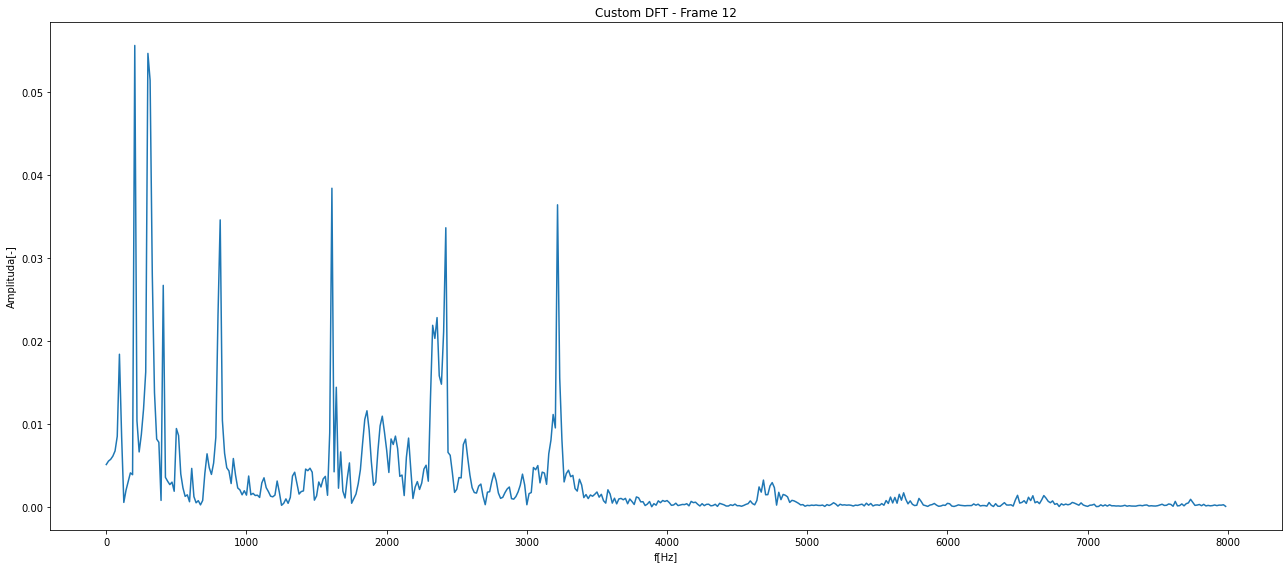
\includegraphics[scale=0.5,keepaspectratio]{Figure_5}
	\caption{Custom implementovaná funkce DFT}
\end{figure}
\end{landscape}

\begin{landscape}
\begin{figure}[H] 
	\centering
	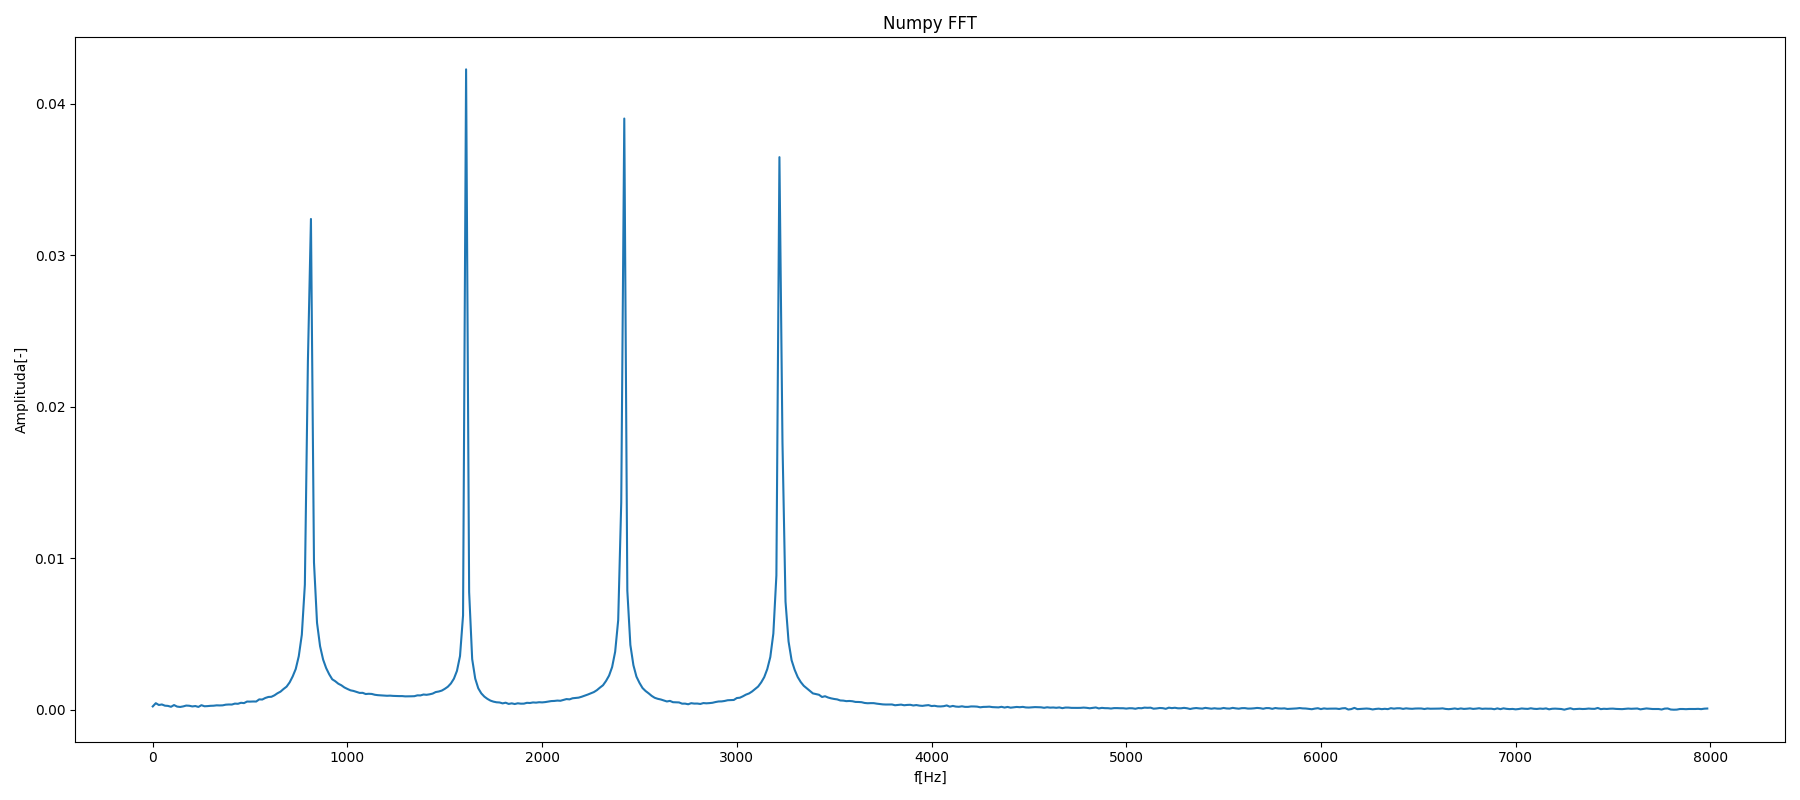
\includegraphics[scale=0.5,keepaspectratio]{Figure_4}
	\caption{Buildin FFT z knihovny numpy}
\end{figure}
\end{landscape}
\section{Spektrogram}

V této části se podíváme na frekvenční složení vstupního signálu. \\
Byl zobrazen spektrogram celého signálu pomocí funkce spektrogram z knihovny scipy a také jeho výkonová spektrální hustota. Místo této funkce by šla použít přímo naše fourierova transformace u předchozího kroku použítá na každý frame, ale bylo by zbytečné ji použít když máme k dispozici přímo funkci, která nám vygeneruje rovnou data celého spektrogramu bez nutnosti dalších operací s daty na naší straně. Další výhodou bude rychlost zpracování, protože tato knihovna je velmi optimalizovaná narozdíl od naší implementace. \\
Pro další krok - určení rušivých frekvencí, byl vytvořen i graf výkonové spektrální hustoty pro první frame signálu (pouze šum).

\begin{figure}[H] 
	\centering
	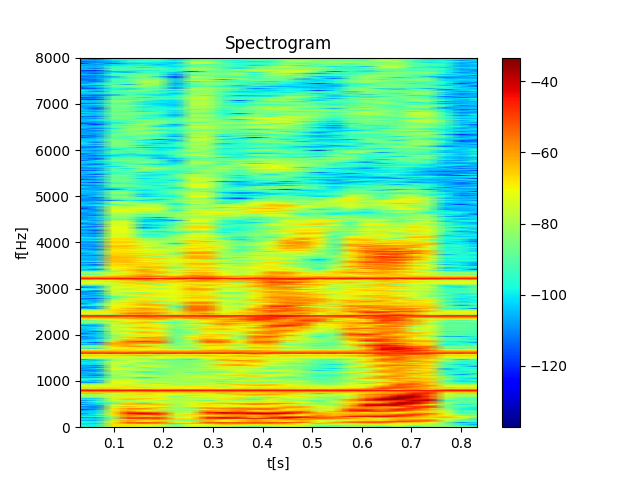
\includegraphics[scale=0.7,keepaspectratio]{Figure_6}
	\caption{Výkonový spektrogram}
\end{figure}

\begin{figure}[H] 
	\centering
	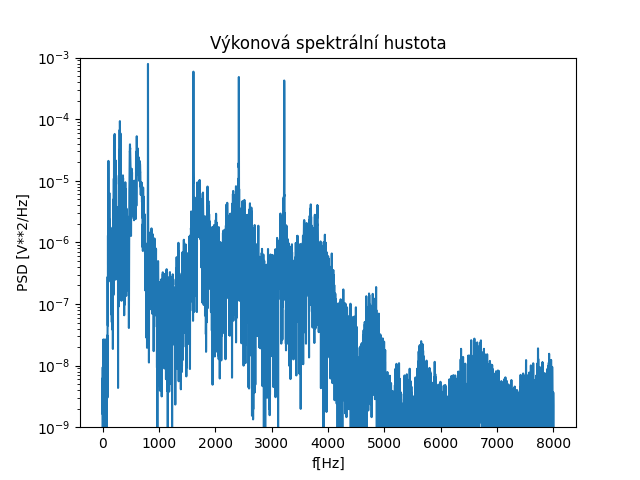
\includegraphics[scale=0.7,keepaspectratio]{Figure_7}
	\caption{Výkonová spektrální hustota}
\end{figure}

\begin{figure}[H] 
	\centering
	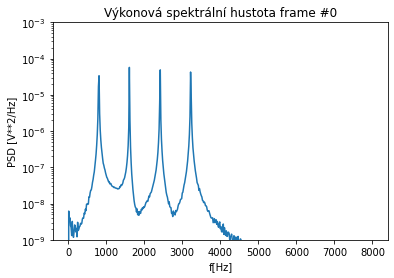
\includegraphics[scale=0.7,keepaspectratio]{Figure_26}
	\caption{Výkonová spektrální hustota frame \#0}
\end{figure}
\section{Určení rušivých frekvencí}
\label{sec:noise_freq}

Z grafů výše můžeme vidět, že peaky rušení jsou +- stejně daleko od sebe, takže můžeme říci že jsou harmonicky vztažené neboli, že frekvence rušení 2., 3., 4., jsou násobky 1.
Z FFT grafu z úlohy 3 můžeme odečíst hodnoty frekvencí peaků, které jsou 3223, 2423, 1615 a 800 Hz.
Dále byla naprogramována funkce na získání frekvencí rušení z výkonové spektrální hustoty.
Funkce má argumenty signál z kterého chceme peaky získat (například spektrální hustota), pole korespondujících frekvencí, počet peaků které chceme najít a šířku pásma v kterém se už nebude hledat kolem peaků.
Potom se podle počtu peaků cyklí a na začátku cyklu získáme index s nejvyšší hodnotou ve vstupním signálu a hledá se k němu korespondující frekvence v poli frekvencí a uloží se do výstupního pole.
Poté se odstraní ze vstupního signálu hodnoty v okolí nalezeného peaku (i s daným peakem) a cyklus začíná od začátku.

Funkce vrátila hodnoty 812.5, 1609.375, 2421.875 a 3218.75 Hz.
Tyto hodnoty se velmi blíží těm co byli odečteny z grafu, takže funkce funguje správně.
Dále můžeme vidět, že tyto frekvence jsou opravdu skoro násobky nejnižší frekvence rušení, je zde ale malá nepřesnost způsobená nejspíš malou vzorkovací frekvencí signálu a tím pádem jeho zkreslením.
\section{Generování signálu}

Byl vygenerován signál obsahující pouze rušení složený z cosinusovek o frekvencích nalezených dříve pomocí funkce np.cos z knihovny numpy. Tento signál byl poté podroben spektrální analýze.
Výsledný signál byl normalizován a byl vytvořen spektrogram a spektrální hustota tohoto signálu.
Tento signál byl následně převeden na 16bit integer (pro uložení v 16bit wav) a uložen. Následně byl tento signál zobrazen v grafu.

\begin{figure}[H] 
	\centering
	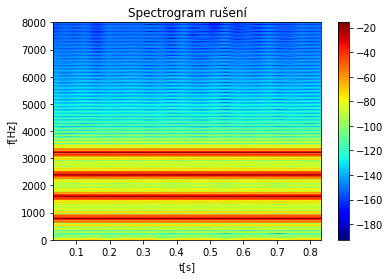
\includegraphics[scale=0.67,keepaspectratio]{Figure_8}
	\caption{Výkonový spektrogram rušení}
\end{figure}

\begin{figure}[H] 
	\centering
	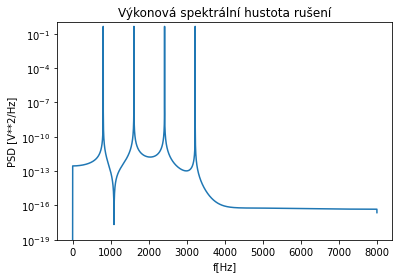
\includegraphics[scale=0.67,keepaspectratio]{Figure_9}
	\caption{Výkonová spektrální hustota rušení}
\end{figure}

\begin{landscape}
\begin{figure}[H] 
	\centering
	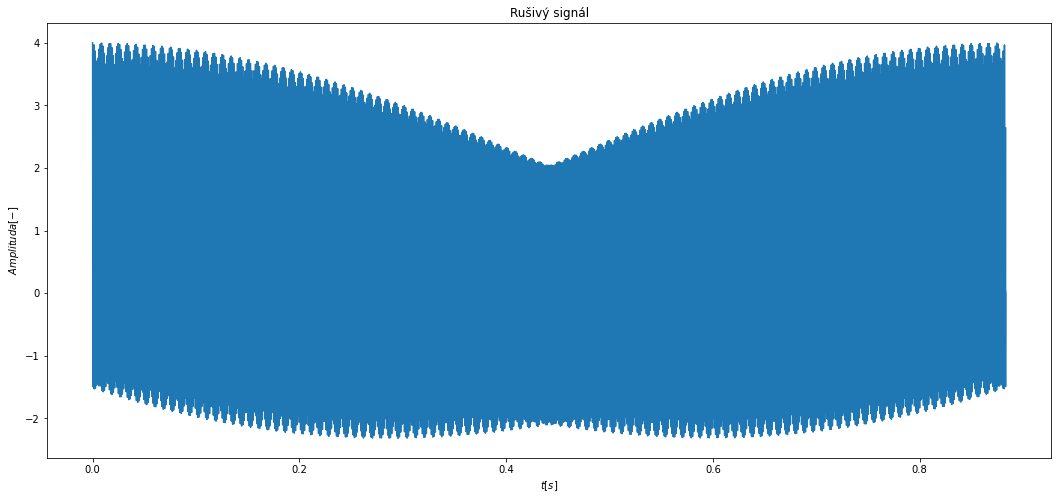
\includegraphics[scale=0.55,keepaspectratio]{Figure_25}
	\caption{Signál rušení}
\end{figure}
\end{landscape}
\section{Čistící filtr}

Byli navrženy 2 sady 4 filtrů typu pásmová zádrž na zablokování rušivých frekvencí (1 pro každou frekvenci).
Z grafů lze vidět, že Butterworthův filtr se po jednotkovém skoku nejrychleji ustálí na 0, ale aplituda zákmitů po před ustálením je vyšší než u Elliptic filtru.

\begin{figure}[H] 
	\centering
	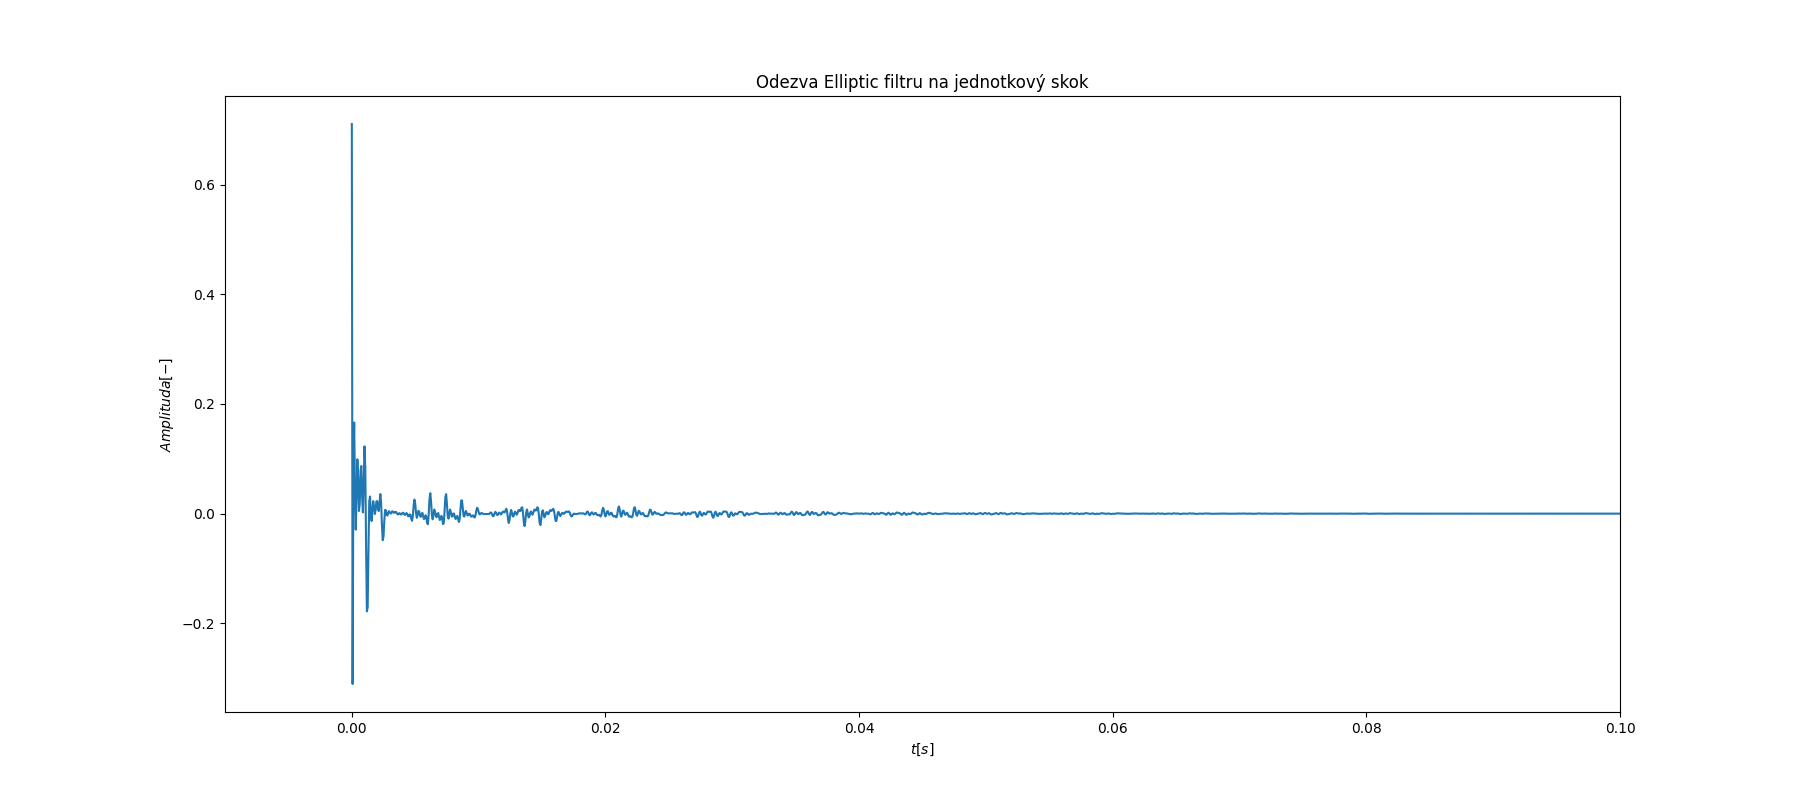
\includegraphics[scale=0.40,keepaspectratio]{Figure_22}
	\caption{Odezva na jednotkový skok Elliptic filtru}
\end{figure}

\begin{figure}[H] 
	\centering
	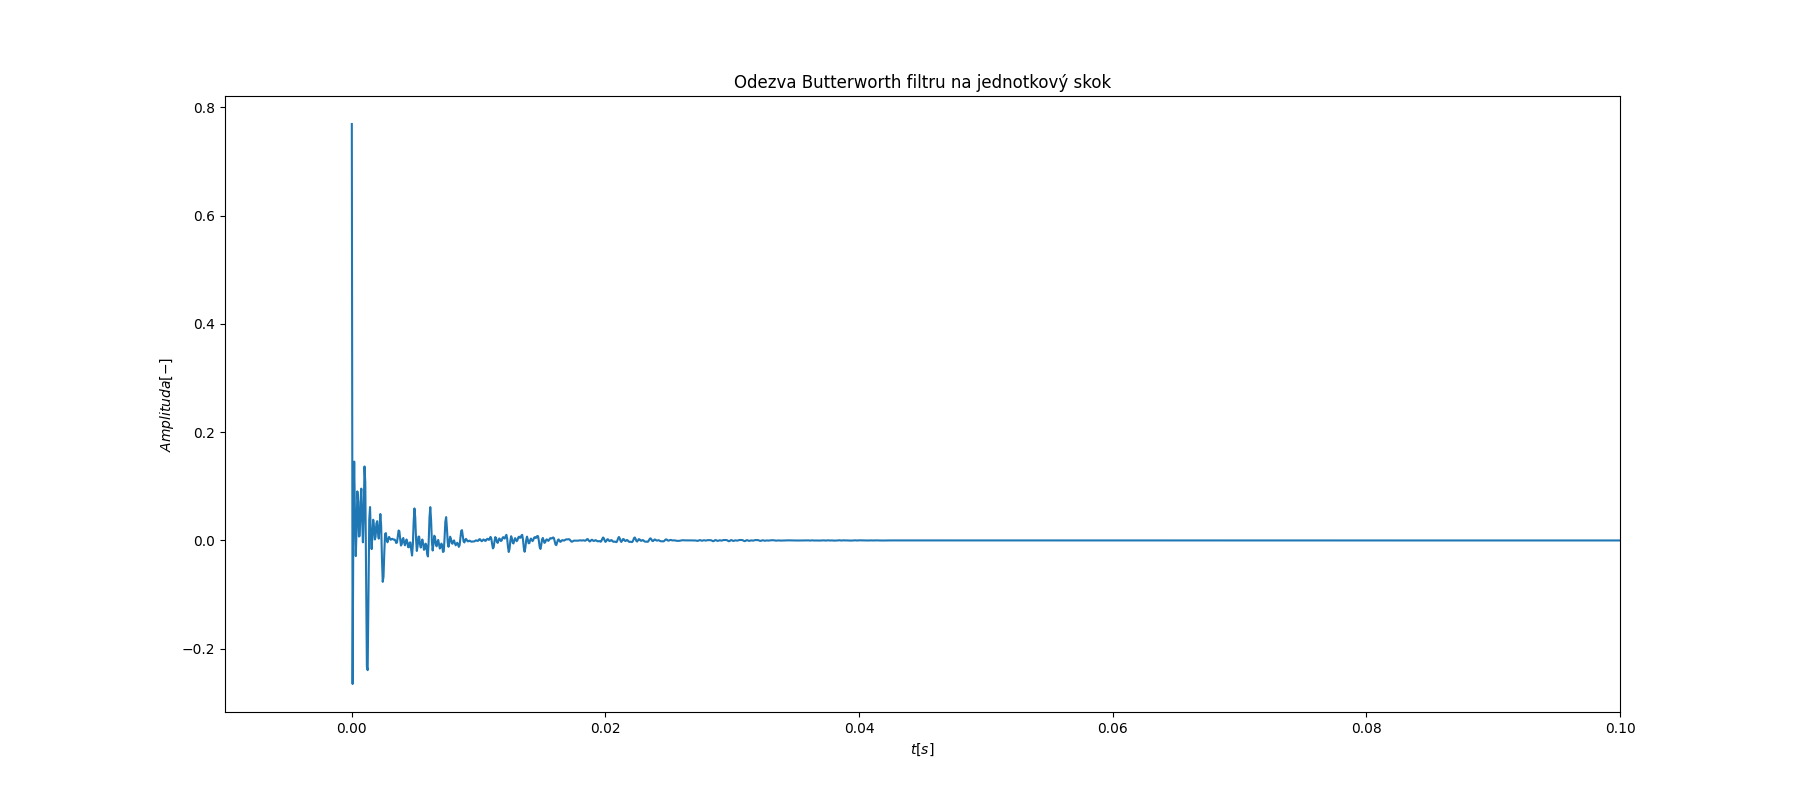
\includegraphics[scale=0.40,keepaspectratio]{Figure_24}
	\caption{Odezva na jednotkový skok Butterworth filtru}
\end{figure}
\section{Nulové body a póly}
Póly a nuly byli získány pomocí funkce "signal.sos2zpk" z dat filtrů a tyto hodnoty byli vykresleny do grafů podle příkladů z \url{https://nbviewer.org/github/zmolikova/ISS_project_study_phase/blob/master/Zvuk_spektra_filtrace.ipynb}.
Navíc byli přidány grafy s detailem na vykreslené body vzhledem k tomu, že tyto body byli tak blízko u sebe že je z nepřiblíženého grafu nelze od sebe skoro rozeznat.

\begin{figure}[H] 
	\centering
	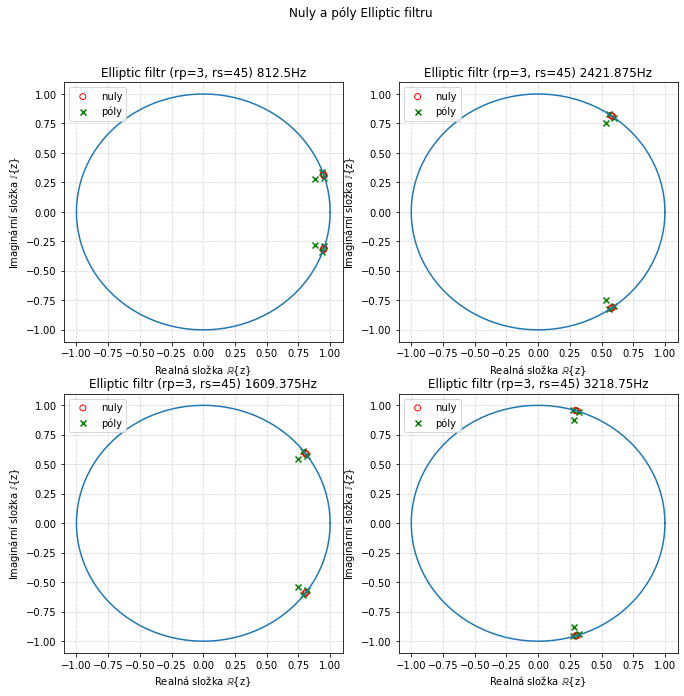
\includegraphics[scale=0.60,keepaspectratio]{Figure_19}
	\caption{Nulové body a póly Elliptic filtrů}
\end{figure}

\begin{figure}[H] 
	\centering
	\includegraphics[scale=0.60,keepaspectratio]{Figure_32}
	\caption{Nulové body a póly Elliptic filtrů (detail)}
\end{figure}

\begin{figure}[H] 
	\centering
	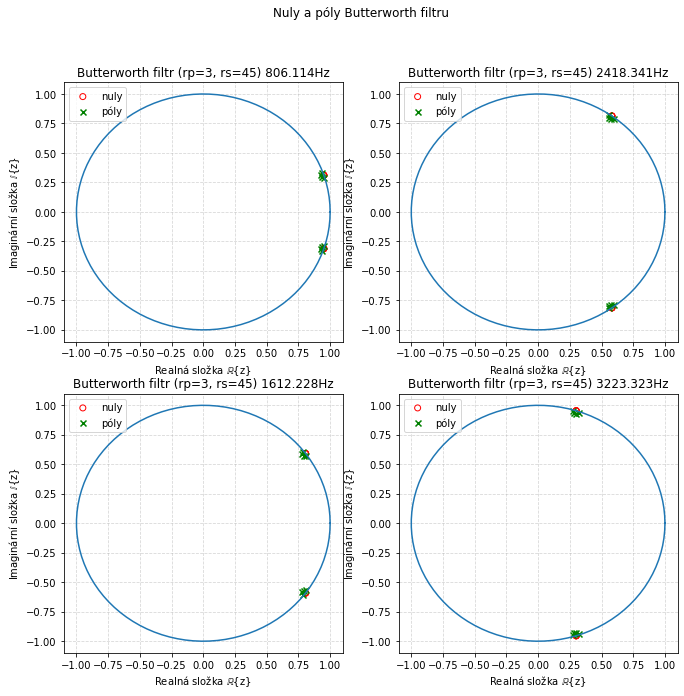
\includegraphics[scale=0.60,keepaspectratio]{Figure_18}
	\caption{Nulové body a póly Butterworthových filtrů}
\end{figure}

\begin{figure}[H] 
	\centering
	\includegraphics[scale=0.6,keepaspectratio]{Figure_31}
	\caption{Nulové body a póly Butterworthových filtrů (detail)}
\end{figure}
\section{Frekvenční charakteristika}

Pro vytvoření frekvenční charakteristiky filtru byla použita funkce "signal.sosfreqz", která z dat filtru vytvoří data frekvenční charakteristiky pro daný filtr.
Tato funkce vrací pole normovaných frekvencí v rozmezí 0 - pi a pole frekvenční odezvy jako komplexní čísla.

Prvním krokem je převod normované frekvence na klasickou frekvenci.
Pro frekvenční odezvu v decibelech jsou hodnoty modulu přepočítány na decibely.
Tyto hodnoty jsou potom zobrazeny v grafu.
Frekvenční charakteristika v modulu a argumentu se liší tím že komplexní čísla odezvy jsou nejdřív převedena na modul pomocí funkce "np.abs" a argument je získán pomocí "np.angle" a graf byl vykreslen podle příkladu na \url{https://nbviewer.org/github/zmolikova/ISS_project_study_phase/blob/master/Zvuk_spektra_filtrace.ipynb}.

Lze vidět že je zde malý rozdíl mezi Butterworth a Elliptic filtrem. Přenos Elliptic filtru klesne skoro o 3dB těsně před přechodem a taky je zde zákmit v záverném směru k -40dB, zatímco Butterworth filtr nic takového nemá, takže pro tento případ by se Butterworth filtr dal považovat za lepší, protože není žádoucí aby klesal přenos v propustném směru před samotným přechodem do závěrného směru a zároveň chceme aby filtr v závěrném směru propouštěl co nejméně.
\subsection{Elliptic filtry}
\begin{figure}[H] 
	\centering
	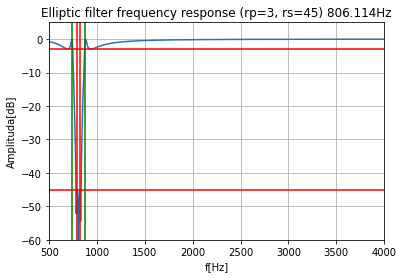
\includegraphics[scale=0.65,keepaspectratio]{Figure_10}
	\caption{Frekvenční odezva Elliptic filtru 1}
\end{figure}

\begin{figure}[H] 
	\centering
	\includegraphics[scale=0.65,keepaspectratio]{Figure_35}
	\caption{Frekvenční charakteristika Elliptic filtru 1}
\end{figure}

\begin{figure}[H] 
	\centering
	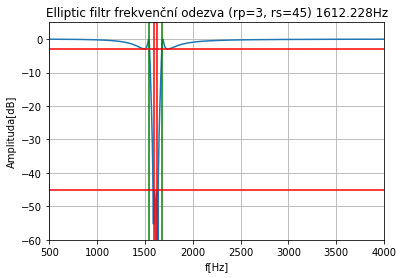
\includegraphics[scale=0.65,keepaspectratio]{Figure_11}
	\caption{Frekvenční odezva Elliptic filtru 2}
\end{figure}

\begin{figure}[H] 
	\centering
	\includegraphics[scale=0.65,keepaspectratio]{Figure_36}
	\caption{Frekvenční charakteristika Elliptic filtru 2}
\end{figure}

\begin{figure}[H] 
	\centering
	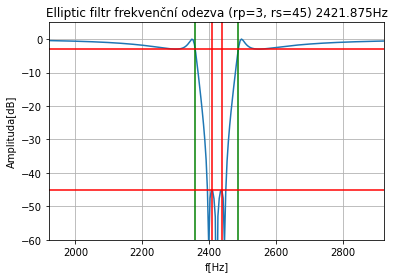
\includegraphics[scale=0.65,keepaspectratio]{Figure_12}
	\caption{Frekvenční odezva Elliptic filtru 3}
\end{figure}

\begin{figure}[H] 
	\centering
	\includegraphics[scale=0.65,keepaspectratio]{Figure_37}
	\caption{Frekvenční charakteristika Elliptic filtru 3}
\end{figure}

\begin{figure}[H] 
	\centering
	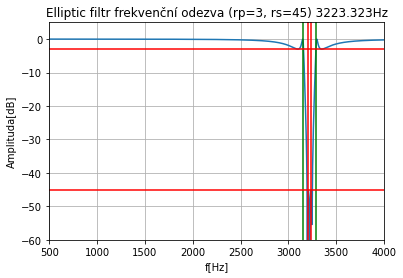
\includegraphics[scale=0.65,keepaspectratio]{Figure_13}
	\caption{Frekvenční odezva Elliptic filtru 4}
\end{figure}

\begin{figure}[H] 
	\centering
	\includegraphics[scale=0.65,keepaspectratio]{Figure_38}
	\caption{Frekvenční charakteristika Elliptic filtru 4}
\end{figure}

\subsection{Butterworth filtry}
\begin{figure}[H] 
	\centering
	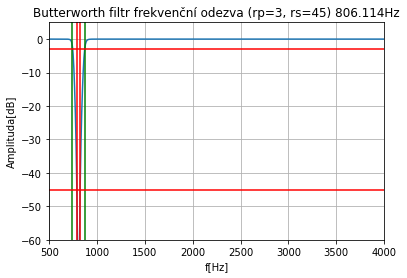
\includegraphics[scale=0.65,keepaspectratio]{Figure_14}
	\caption{Frekvenční odezva Butterworth filtru 1}
\end{figure}

\begin{figure}[H] 
	\centering
	\includegraphics[scale=0.65,keepaspectratio]{Figure_39}
	\caption{Frekvenční charakteristika Butterworth filtru 1}
\end{figure}

\begin{figure}[H] 
	\centering
	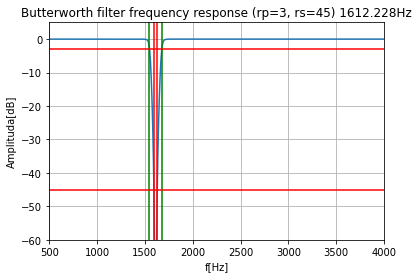
\includegraphics[scale=0.65,keepaspectratio]{Figure_15}
	\caption{Frekvenční odezva Butterworth filtru 2}
\end{figure}

\begin{figure}[H] 
	\centering
	\includegraphics[scale=0.65,keepaspectratio]{Figure_40}
	\caption{Frekvenční charakteristika Butterworth filtru 2}
\end{figure}

\begin{figure}[H] 
	\centering
	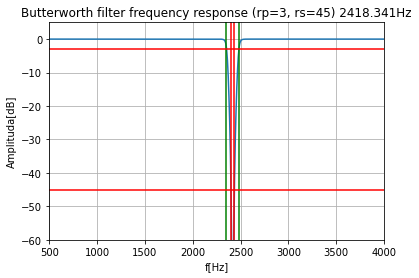
\includegraphics[scale=0.65,keepaspectratio]{Figure_16}
	\caption{Frekvenční odezva Butterworth filtru 3}
\end{figure}

\begin{figure}[H] 
	\centering
	\includegraphics[scale=0.65,keepaspectratio]{Figure_41}
	\caption{Frekvenční charakteristika Butterworth filtru 3}
\end{figure}

\begin{figure}[H] 
	\centering
	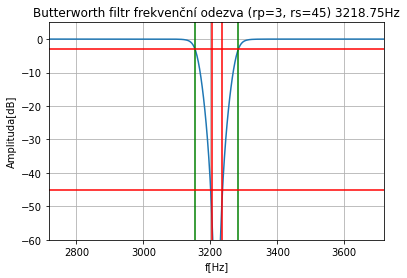
\includegraphics[scale=0.65,keepaspectratio]{Figure_17}
	\caption{Frekvenční odezva Butterworth filtru 4}
\end{figure}

\begin{figure}[H] 
	\centering
	\includegraphics[scale=0.65,keepaspectratio]{Figure_42}
	\caption{Frekvenční charakteristika Butterworth filtru 4}
\end{figure}
\section{Filtrace}
\subsection{Elliptic filtry}
\begin{figure}[H] 
	\centering
	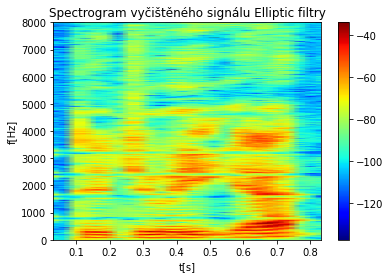
\includegraphics[scale=0.65,keepaspectratio]{Figure_20}
	\caption{Výkonový spektrogram vyčištěného signálu Elliptic filtry}
\end{figure}

\begin{figure}[H] 
	\centering
	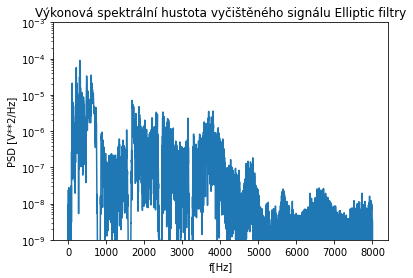
\includegraphics[scale=0.65,keepaspectratio]{Figure_21}
	\caption{Výkonová spektrální hustota vyčištěného signálu Elliptic filtry}
\end{figure}

\begin{landscape}
\begin{figure}[H] 
	\centering
	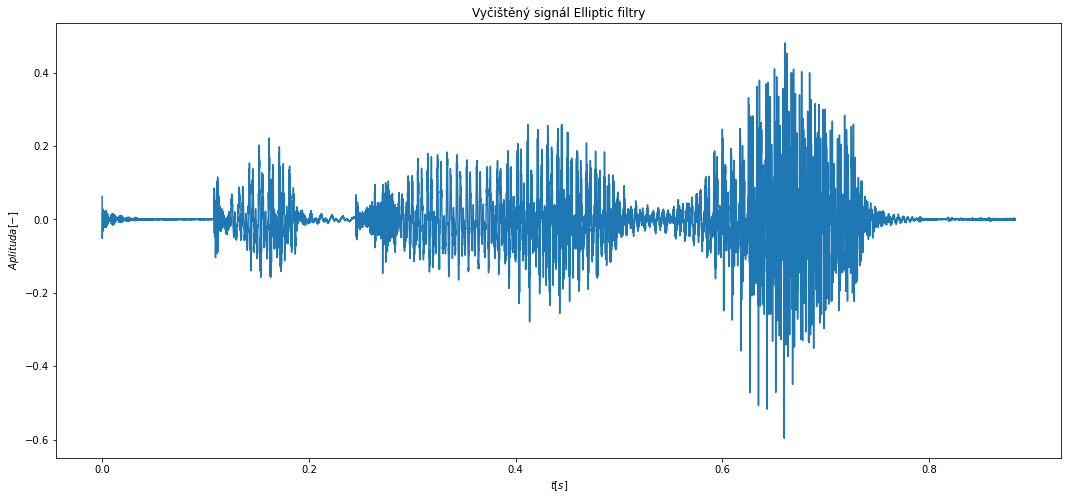
\includegraphics[scale=0.55,keepaspectratio]{Figure_23}
	\caption{Výsledný vyčištěný signál Elliptic filtry}
\end{figure}
\end{landscape}

\subsection{Butterworth filtry}
\begin{figure}[H] 
	\centering
	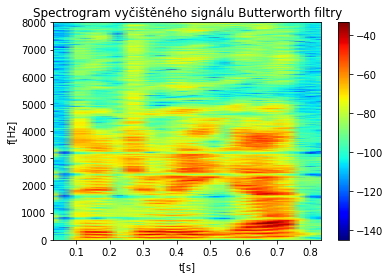
\includegraphics[scale=0.65,keepaspectratio]{Figure_27}
	\caption{Výkonový spektrogram vyčištěného signálu Butterworth filtry}
\end{figure}

\begin{figure}[H] 
	\centering
	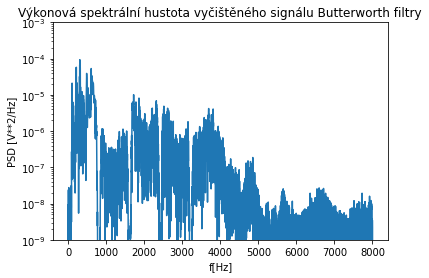
\includegraphics[scale=0.65,keepaspectratio]{Figure_28}
	\caption{Výkonová spektrální hustota vyčištěného signálu Butterworth filtry}
\end{figure}

\begin{landscape}
\begin{figure}[H] 
	\centering
	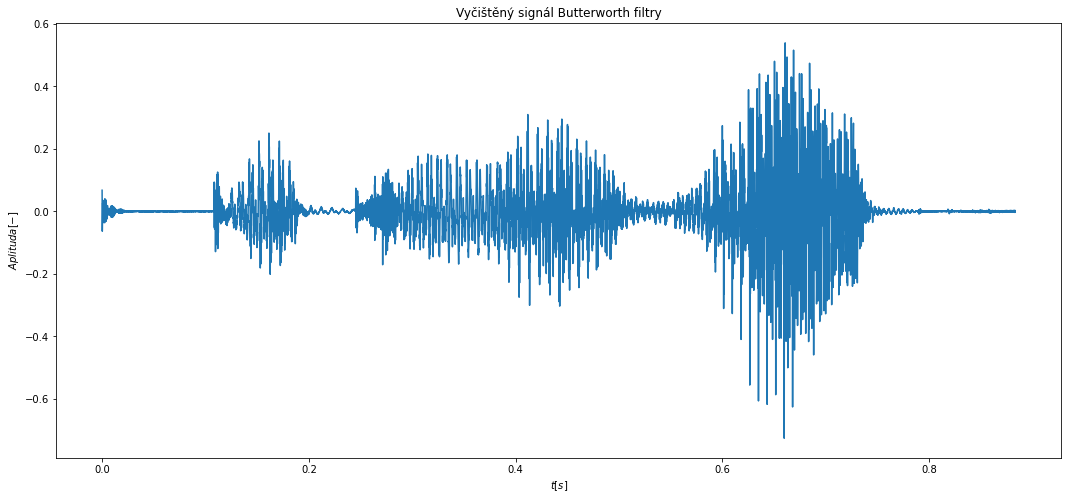
\includegraphics[scale=0.55,keepaspectratio]{Figure_29}
	\caption{Výsledný vyčištěný signál Butterworth filtry}
\end{figure}
\end{landscape}

\subsection{Shrnutí filtrace}
Vzhledem k tomu že se Butterworthův i Elliptic filtr chovali téměř identicky nebylo potřeba provádět čištění oběma.
Na výsledné číštění byl ale nakonec použit Elliptic filtr protože méně zkresluje signál na začátku a na konci.\\
Na spectrogramu vyčištěného signálu již nevidíme tak výrázné rušení i když nějaké rušení zde stále zůstalo. To může být způsobeno povahou rušení a nebo chováním filtru kde nemá na začátku ještě dostatek vzorků pro analýzu.
Můžeme vidět že i samotný signál je trochu zdeformovaný, což se dalo očekávat, jelikož část frekvenčního spektra tohoto signálu ležela ve stejné oblasti jako odstraňovaný šum.

\begin{landscape}
	\begin{figure}[H] 
		\centering
		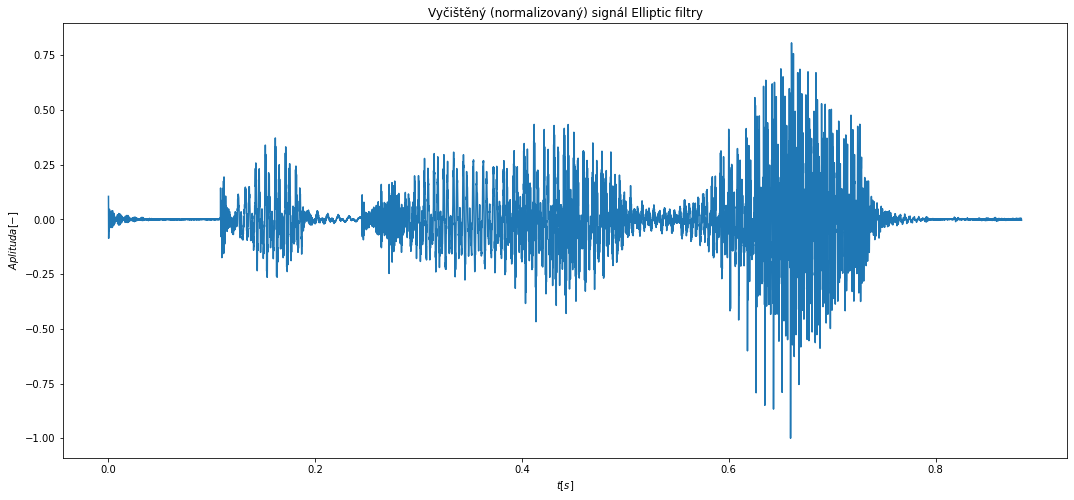
\includegraphics[scale=0.55,keepaspectratio]{Figure_30}
		\caption{Finální vyčištěný signál}
	\end{figure}
\end{landscape}
\section{Experiment filtrace neuronovou sítí}

V této části, která je mimo oficiální zadání, se testuje možnost filtrace pomocí neuronových sítí.
Před vytvořením prvního prototypu, který byl schopen vytvořit aspoň nějaký signál bylo potřeba určit jaká data bude vůbec neuronová síť zpracovávat.
Po několik experimentech bylo určeno, že vstupní data budou normalizované hodnoty 4096 raw hodnot signálu, výstup fourierovy transformace této části signálu a vzorkovací frekvence.
Jako dataset byli použity stažené mp3 audio stopy náhodných youtube videí, které byli následně převedeny na wav formát a normalizovány na hodnoty -1 - 1, poté zarušeny náhodným rušením (náhodná amplituda 0 - 4, s náhodnou frekvení 0 - 48kHz a náhodnou fází).
Pro zjištění výkonu neuronové sítě byl využit ukazatel MSE (Mean Square Error - průměrná střední odchylka) a SNR (Signal to Noise Ratio).

\subsection{Prototyp 1}

První prototyp byl schopný vytvořit aspoň nějaký signál, který vypadá že je bez rušení, ale zároveň nebyla neuronová sít schopná zreplikovat ani dobrou část signálu.
Toto chování bude nejspíš způsobeno kapacitou neuronové sítě - pro testování učícího scriptu byl vytvořen pouze malý model, aby bylo trénování rychlé.
Po 5.5h trénování byla dosažena maximální kapacita modelu (validační SNR dále nerostlo) a tak bylo trénování tohoto prototypu ukončeno.
Tento model se byl schopný dostat na SNR 30, což není vůbec špatná, ale u audio signálů je tato hodnota stále příliš malá.

Jako model byl použit malý autoencoder pro 1D data s residuálními spoji, které zaručují lepší propagaci nezpracovaných dat dále do model.
Množství trénovatelných parametrů tohoto modelu je 35M, takže tento model není úplně malý, ale je to hlavně způsobeno rozměrem vstupních dat.

\begin{figure}[H] 
	\centering
	\includegraphics[scale=0.25,keepaspectratio]{model_1.png}
	\caption{Konstrukce modelu neuronové stítě prototypu 1}
\end{figure}

\begin{landscape}
\begin{figure}[H] 
	\centering
	\includegraphics[scale=0.6,keepaspectratio]{Figure_33.png}
	\caption{Vyčištěný signál s použitím neuronové sítě prototypu 1}
\end{figure}
\end{landscape}

\end{document}